
\section{Results and Discussions}
\label{section:results}

In this section, I present and discuss the main regression results on the effect of the number of children on different outcomes. I will first present and discuss the main regression estimates found using the whole population of firstborns (2+ sample) and the population of first- and second-borns (3+ sample), which are reported in \autoref{tab:main-res}. The subsections that follow discuss possible challenges to the validity of the instruments used and whether there is effect heterogeneity with respect to the characteristics of the mother.


%Tex File: D:/R_projects/MScED_Dissertation/tex/tables/main-res.tex

% Date and time: Fri, May 13, 2022 - 2:58:39 PM
\begin{sidewaystable}[!htbp] \centering 
  \caption{OLS and 2SLS Estimates of The Effect of The Number of Children} 
  \label{tab:main-res} 
\begin{threeparttable}
\begin{tabular}{@{\extracolsep{5pt}}lcccccccc} 
\\[-1.8ex]\hline 
\hline \\[-1.8ex] 
 & \multicolumn{4}{c}{2+ Sample} & \multicolumn{4}{c}{3+ Sample} \\
\cline{2-5}  \cline{6-9} \\
 & OLS & \multicolumn{3}{c}{2SLS} & OLS & \multicolumn{3}{c}{2SLS} \\ 
\cline{3-5}  \cline{7-9} \\[-1.8ex]
\\[-1.8ex] & (1) & (2) & (3) & (4) & (5) & (6) & (7) & (8)\\ 
\hline \\[-1.8ex] 
 Educational Attainment & $-$0.006$^{***}$ & 0.005 & $-$0.013 & 0.004 & $-$0.008$^{***}$ & 0.012 & 0.052$^{*}$ & 0.016$^{*}$ \\ 
  & (0.001) & (0.006) & (0.023) & (0.006) & (0.001) & (0.009) & (0.028) & (0.008) \\ 
  & & & & & & & & \\ 
 Left Behind & 0.023$^{***}$ & $-$0.004 & 0.084 & 0.001 & 0.025$^{***}$ & $-$0.025 & $-$0.025 & $-$0.025 \\ 
  & (0.002) & (0.019) & (0.074) & (0.018) & (0.003) & (0.025) & (0.078) & (0.024) \\ 
  & & & & & & & & \\ 
 Private School & $-$0.003$^{***}$ & $-$0.017 & $-$0.021 & $-$0.017$^{*}$ & $-$0.003$^{**}$ & 0.010 & $-$0.025 & 0.007 \\ 
  & (0.001) & (0.011) & (0.041) & (0.010) & (0.001) & (0.016) & (0.047) & (0.015) \\ 
  & & & & & & & & \\ 
 Mothers LFP & $-$0.019$^{***}$ & $-$0.021 & 0.027 & $-$0.019 & $-$0.023$^{***}$ & 0.038 & 0.112 & 0.045 \\ 
  & (0.002) & (0.016) & (0.061) & (0.015) & (0.003) & (0.030) & (0.093) & (0.028) \\ 
  & & & & & & & & \\ 
\hline \\[-1.8ex] 
IV used & - & Twins2 & Boy12 & Twins2, Boy12 & - & Twins3 & Boy123 & Twins3, Boy123 \\ 
  &   &   & Girl12 & Girl12 &   &   & Girl123 & Girl123 \\ 
\hline 
\hline \\[-1.8ex] 
\end{tabular} 
\begin{tablenotes}
\footnotesize
\item \textit{Notes:} Covariates for all models include age 
(in months) and sex of child, mother's characteristics (education, ethnicity, age during
census, age at first birth, and income range), dummies for districts, and a dummy for whether the father 
resides in the household. The regressions for the 3+ sample are clustered by mother's ID.
The regressions using the SameSex12 and SameSex123 instruments were excluded for reasons 
of space. The results are qualitatively similar to the ones in columns 3 and 7, 
respectively, and are available upon request. Robust standard errors are in parentheses. 
*** Significant at 1\%, ** Significant at 5\%, * Significant at 10\%.
\end{tablenotes}
\end{threeparttable}
\end{sidewaystable} 





\autoref{tab:main-res} presents OLS and 2SLS estimates of the effect of the number of children on the four outcome variables discussed in Section \ref{section:outcomes}. OLS results, reported in column 1 (for the 2+ sample) and column 5 (for the 3+ sample), point to the expected negative association between family size and favourable outcomes.These results correspond to the standard pattern: children who grow up in larger families have lower educational attainment, are more likely to be left behind in school, and are less likely to attend private school. Mothers are also less likely to participate in the labour market when they have many children. It is also important to point out that these estimates are very precise: their standard errors range from .001 to .003. However, these results are only indicative and, in the presence of possible endogeneity of family size, cannot be taken as showing causality.

In contrast to the OLS results, 2SLS estimates consistently point to a statistically insignificant or even positive effects of family size. The 2SLS results using Twins instruments are shown in column 2 (for the 2+ sample) and column 6 (for the 3+ sample) of \autoref{tab:main-res}. All of the estimates are statistically insignificant at conventional levels and even some have unexpected signs. For example, the effect on the educational attainment index in the 2+ sample using Twins2 as an IV is .005 (se = .006) while the corresponding effect in the 3+ sample (using Twins3 as an IV) is .012 (se = .009). Similarly, the 2SLS estimates of the impact on the dummy variable \enquote{Left Behind} are statistically insignificant and have the unexpected signs in both the 2+ and 3+ samples. The lack of statistical significance using twins instruments also extend to the variables that relate to child investment, that is, private school attendance and the mother's labour force participation. 

Similar results hold when using sex composition instruments. 2SLS estimates using both Boy12 and Girl12 instruments (column 3 of \autoref{tab:main-res}) show no effect of the number of children on any of the outcomes. Similar results hold in the 3+ sample when using Boy123 and Girl123 instruments together (column 7 of \autoref{tab:main-res}). The only exception is the effect on educational attainment [0.052 (se = 0.028)], which surprisingly, has an unexpected sign and is statistically significant only at the 10\% level. The results for the probability of being left behind in the 3+ sample and mothers' labour force participation in both samples, although insignificant, also have the opposite signs to the OLS estimates. It is also worth noting that the standard errors of the estimates obtained using sex composition instruments are substantially higher than the corresponding standard errors for the twins instruments in all of the estimated models.

Columns 4 and 8 of \autoref{tab:main-res} report 2SLS results using an instrument list that combines the twins and sex composition instruments in each sample. The purpose of combining these two different sets of instruments is to increase precision and thereby produce a single more efficient IV estimate \parencite{angrist_multiple_2010}. Indeed, the standard errors of the estimates in column 4 (2+ sample) and column 8 (3+ sample) are lower than the corresponding estimates using each group of instruments separately (columns 2 and 3 for the 2+ sample; and columns 6 and 7 for the 3+ sample). The estimates obtained using the combined instruments bolsters the null results that is obtained using each instrument set separately: none of the estimates obtained are statistically significant at the 5\% level and only two results are significant at the 10\% level. The estimate for the effect on educational attainment in the 3+ sample [0.016 (se = 0.008)], although significant at the 10\% level, has an unexpected sign. The effect on private school attendance in the 2+ sample, which is $ -0.017 $ (se = 0.010), is the only other estimate that is significant at the 10\% level.

As discussed in Section \ref{section:IVs}, the two sets of instruments capture an average causal response for different subpopulation of compliers. We have also shown that each instrument shifts the fertility distribution very differently (see \autoref{fig:acrs}). Now, given the similar set of 2SLS estimates they generate, one wonders if these results are pointing to a homogenous effect, i.e., a common family size effect of zero for just about everybody. I conducted an overidentification test to formally test the equality of the 2SLS estimates generated by the two sets of instruments. The test results (not presented, but available upon request) show that we cannot reject the null of equality of the estimates for the two instrument sets across all of the outcomes in both samples. In this setting, the traditional overidentification test becomes a formal test for treatment effect homogeneity.\footnote{ Homogeneity of results is also a strong indication of the external validity of the results \parencite[see][p.~776]{angrist_multiple_2010}. Thus, the overidentification test also serves to assess, to some extent, external validity. } But, as \textcite[p.~167]{Angrist2009} point out, this requires maintaining the hypothesis that all instruments in the overidentified model are valid, a topic we turn to next.


\subsection{Validity of the Instruments}
\label{section:valid}

A very important consideration in any IV study is validity. Following the ACR framework, anything that affect the randomness of our instruments and/or causes the exclusion restriction to fail is a threat to validity. In such a case, 2SLS estimates become biased and inconsistent. In this subsection I discuss various challenges to the randomness of both instruments and ways I tried to address them.

One concern with the randomness of twin births is that it might be related to family background characteristics. There is a common finding that older mothers are more likely to give birth to twins than younger mothers. I find this to be also the case in the 2+ sample but not in the 3+ sample. Mothers who give birth to twins during their second birth are about a year older at first birth compared to mothers who don't in the 2+ sample. In order to address this, I run separate regressions (both OLS and 2SLS) after splitting the 2+ sample based on intervals of the mother's age at first birth. The estimates, along with their 95\% confidence intervals are plotted in \autoref{fig:age-mods}. The general picture reveals that the results remain qualitatively the same across all age ranges, suggesting that systematic biases due to the age of the mother is not a concern. In particular, the 2SLS estimates for the \enquote{older mothers} ($ \geq 30 $ years old at first birth) as well as the \enquote{younger mothers} (less than 30 years old at first birth) show no statistically significant impact of the number of children on virtually any of the outcomes. The only exception is the effect on educational attainment for the 30+ sample, but this is barely significant (imprecisely estimated) and has the opposite sign to the OLS estimate. 

\begin{figure}[!th]
\centering
\caption{\label{fig:age-mods}Plot of Coefficient Estimates and 95\% CI by Intervals of the Mother's Age at First Birth (2$ + $ Sample)}
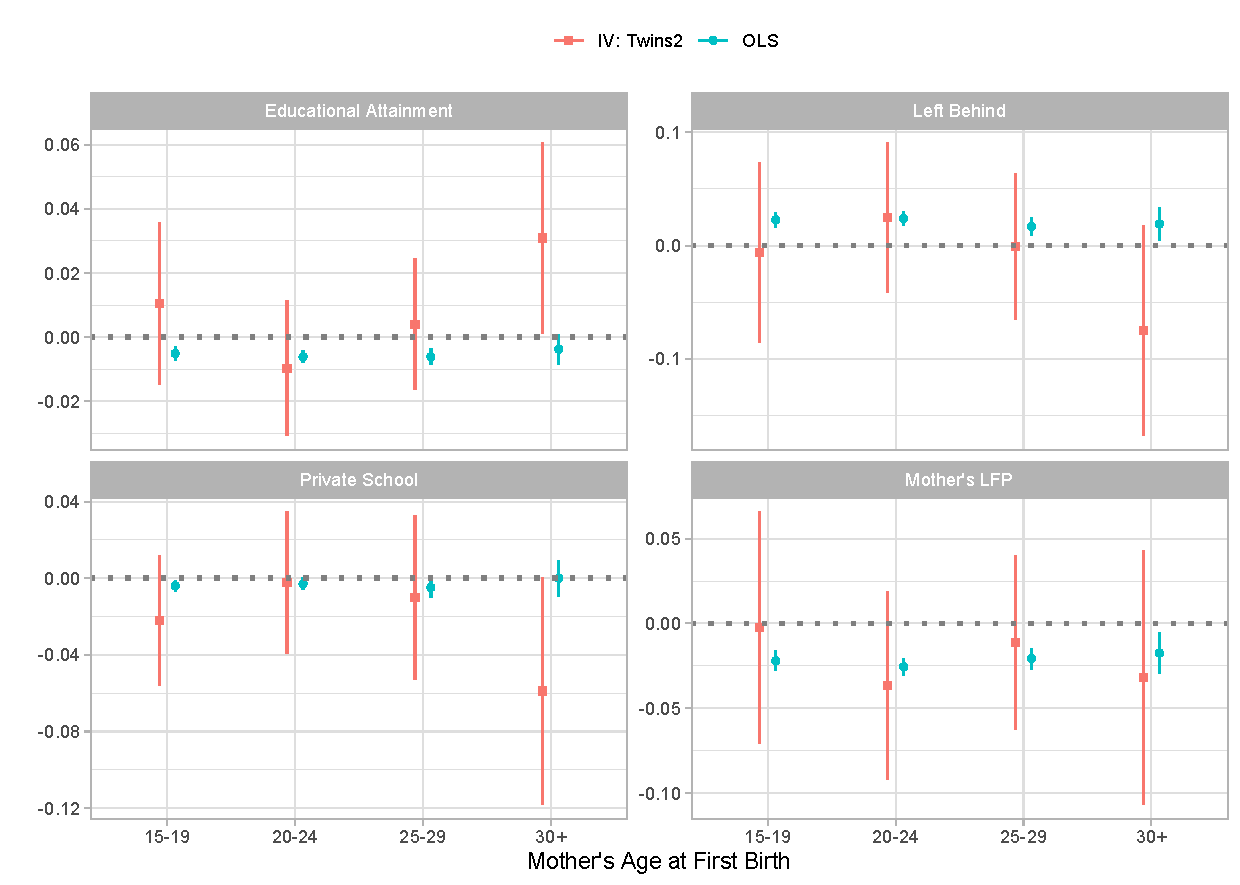
\includegraphics[width=\textwidth]{figures/age_mods.pdf}
\fnote{\textit{Notes:} Each regression was run controlling for the same set of covariates as in \autoref{tab:main-res} for the 2+ sample (see notes there). The sample sizes for each age range are as follows: 24,414 (15-19); 35,125 (20-24); 23,864 (25-29); and 10,021 (31+). Mothers who were younger than 15 at first birth were excluded from the analysis.}
\end{figure}

Another challenge to randomness of twins is the observation that mothers who use fertility enhancing treatments are more likely to have multiple births. Since the use of fertility enhancing treatments is usually unobservable, there is a potential bias from using twin births as an instrument \parencite{braakmann_reconsidering_2016}. Although availability and utilization is low, Assisted Reproductive Technologies (ARTs), such as in vitro fertilizations (IVFs), are becoming more prevalent in South Africa. In fact, South Africa has the second highest number of registered IVF centres in the whole continent in 2019 \parencite{Ombelet2019}. Studies analysing ART registry data from sub–Saharan Africa have observed high multiple pregnancy rates associated with the utilization of ART \parencite{Botha2018,Dyer2019}. There are also indications of a rise in the number of multiple births over time in our data set that could be associated with the evolution of ARTs. Using the dates of births of all respondents in the 2011 South African Census, I plotted the number of multiple births (i.e., twins, triplets, quadruplets, etc.) per 1000 live births from 1970 onwards. This is shown in \autoref{fig:line-pp}. Although there is no historical data on the utilization of ART in South Africa since its introduction in the 1980s (ART registries were established in the early 2000s), the rising trend of multiple births across all population groups is consistent with the introduction and (slow) dissemination of fertility treatments. The figure also indicates the rising disparity in twinning probabilities between white and non-white South Africans (more on this below).

%\begin{figure}[!th]
%\centering
%\caption{\label{fig:line-pp}Multiple Births Per 1000 Live Births by Mother's Population Group}
%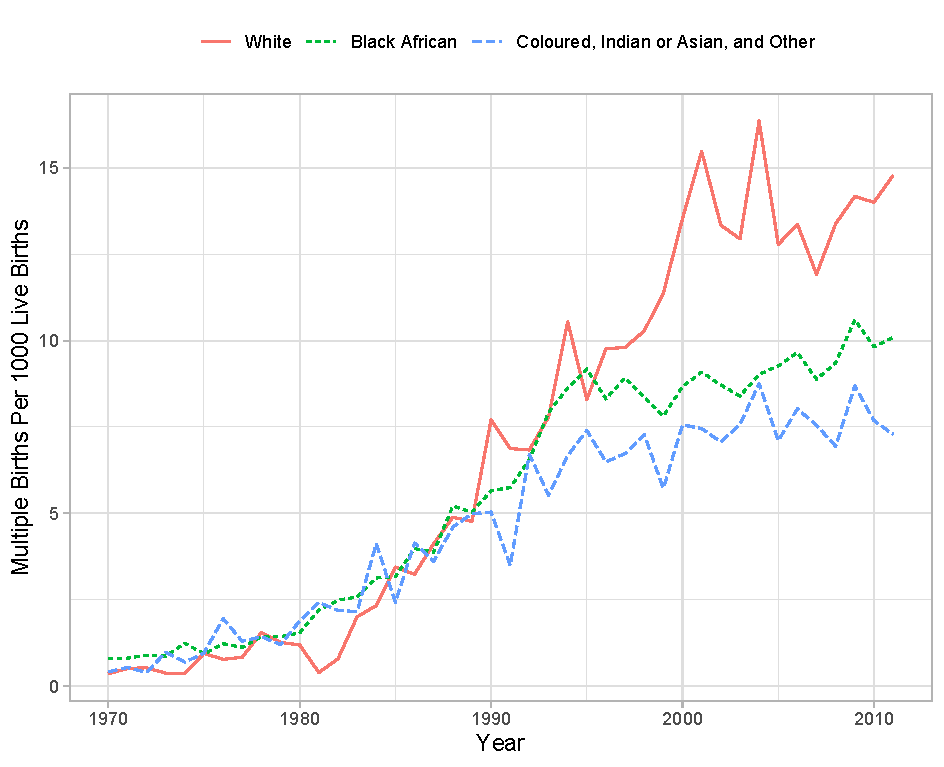
\includegraphics[width=\textwidth]{figures/line_pp.pdf}
%\end{figure}

A related threat to the randomness of twin births is the observation that the occurrence of twins is related to the mother's health and health related behaviour. \textcite{bhalotra_twin_2019} show that twinning is strongly related to morbidity, smoking status, availability of reproductive health services and other health indicators even for mothers not using fertility treatments. They also show that the education of the mother is positively associated with twinning, consistent with the hypothesis that educated women are more likely to engage in health seeking behaviour (as well as to seek fertility enhancing treatments). Although the 2011 South African census does not have data on health indicators, there are indications that twinning is more likely in subpopulations that are more likely to seek health treatments. \autoref{fig:line-pp} reveals that starting from the mid-1990s the occurrence of multiple births is systematically higher among white South Africans as compared to non-whites. This would make sense as white mothers arguably have both the awareness and the capacity with respect to utilizing health treatments, including ARTs. 

To check whether this systematic difference poses a challenge, in each sample, I estimated both OLS and 2SLS regressions using the relevant twins instrument for white and non-white families separately. The results are reported in \autoref{tab:whites-nonwhites}. As can be clearly seen, none of the 2SLS estimates are statistically significant for either whites or non-whites in both samples. Moreover, the signs of the 2SLS estimates, although insignificant and sometimes unexpected, agree for most outcomes. In general, the results are robust to division by mothers' population group, suggesting that there is no evidence of a potential bias stemming from systematic differences in the occurrence of multiple births. Perhaps, the only noteworthy difference is that the correlation between the number of children and the outcomes as captured by the OLS estimates is weaker and usually absent for whites. This, in particular, is clearly observed in the 3+ sample, where almost none of the OLS coefficients are statistically significant at conventional levels. For non-whites, on the other hand, all of the OLS coefficients have their expected signs and are highly significant. 

\textcite{rosenzweig_population_2009} point out a further challenge to the exogeneity of twin births. They argue that the occurrence of twins changes the behaviour of parents in such a way that they reallocate resources away from twins and towards older singleton children. They point out two aspects of twins that affect inter-child allocations: \enquote{(i) the closer spacing of twins, which makes investing in the average quality of the twins more costly compared with investing in non-twins, and (ii) the lower endowments of twins, which will affect the resources allocated to non-twins depending on whether parents reinforce or compensate for endowment differences across children.} \parencite[1152]{rosenzweig_population_2009}.\footnote{ Here, the lower endowment of twins refers to the fact that twins usually have lower birth weight, lower survival rate, lower cognitive achievement, and so on. } If such resource reallocation is taking place, then, they claim, estimates using twins as an instrument will be biased towards zero.

Following \textcite{angrist_multiple_2010}, I estimated reduced-form twins effects on outcomes in samples in which twins are unlikely to affect family size (i.e., there is no first stage) to see if resource reallocation is a problem. The rationale for focusing on no-first-stage samples is that because the birth of twins has no effect on family size in these subsamples, effects of confounding factors related to twinning should surface. The two subsamples with a zero first stage are those from families with closely spaced births ($ <2 $ years between the first two births) and those whose mothers were not educated, both from families with at least three children in the 2+ sample.\footnote{ These are households who are likely to have large families anyway. In such a case, the birth of twins is likely to have little or no effect on family size. }  Columns 1 and 2 in Panel A of \autoref{tab:reduced} shows that the first stage regressions in such families yield insignificant coefficient estimates at the conventional 5\% level. Panel B presents estimates of reduced form regressions for all four outcome variables using the Twin2 IV. If what \textcite{rosenzweig_population_2009} propose is true, we ought to see that older singletons have better outcomes in these no-first-stage samples. But that is simply not the case: in both subsamples, twin births have an insignificant effect (at the 5\% level) on any of the outcomes for older children. The only exception is the probability of private school attendance in the subsample of uneducated mothers (column 2). But even in this case, firstborn children have \textit{lower}, not higher, likelihood of attending private school, in defiance of the hypothesis that non-twin firstborn children are favoured. Hence, there is no evidence for a reallocation effect that could potentially confound our IV estimates.\footnote{ \textcite{Black2010} reached the same conclusion using data on the birth weight of individuals in Norway. In contrast to the critique by \textcite{rosenzweig_population_2009}, they noted that taking account of endowments actually \textit{reduces} the negative effects of family size, a result, they claimed, \enquote{is consistent with compensating rather than reinforcing parental investments} \parencite[p.~35]{Black2010}. } 
  
A similar concern with sex composition instruments is that it might be correlated with background characteristics of the parents. To test this, I estimated a regression of the same-sex instruments in each of the 2+ and 3+ samples (where the first two children are of the same-sex) on the full set of covariates, including characteristics of the mother. The results show no relationship between any of the mother’s background characteristics or other variables and the SameSex12 instrument in the 2+ sample. Only two variables (out of a total of 79) that correspond to the income group of the mother are found to be significant in the 3+ sample regression. But this is not a concern as we condition on these variables in the 2SLS estimation.

One objection to the exclusion restriction with respect to the same-sex IV is that there is a possibility of gender-specific economies of scale (for example, sharing of rooms and/or clothes) that could reinforce child quality investments when parents have children of the same-sex \parencite{clarke_children_2018}. \textcite{rosenzweig_natural_2000} point out that cost efficiencies associated with gender mix will confound the effect of an exogenous increase in the number of children with direct child-rearing cost effects on outcomes. To test this, I run reduced form regressions on subsamples with zero first stages, similar to the no-first-stage analysis for the twins instrument discussed earlier. I consider outcomes for firstborn boys in the 2+ sample, so the appropriate instrument to consider would be the Boy12 dummy. The two subsamples include mothers with less than 2 years of spacing between the first two births and those with no schooling. The results, which are reported in columns 3 and 4 of \autoref{tab:reduced}, show that there is no reduced form relation between the Boy12 instrument and any of the outcomes for the firstborn child. That is, a firstborn male child who has a younger sibling of the same gender does not appear to benefit in anyway as suggested by the same-sex cost advantage hypothesis.\footnote{ The only statistically significant effect is observed on the mother's labour force participation in the subsample with close spacing (column 3). But we are focusing here on the direct effects on the child’s outcomes. Even though there would be indirect effects, we should have seen it in the regressions where child outcomes are the dependent variables. } Hence, there is no ground to suspect a violation of the exclusion restriction based on household efficiencies related to same-sex sibships. 


\subsection{Heterogeneity Analysis}

A natural question in any causal analysis is whether the treatment effect varies with covariates, such as age, ethnicity, etc. This kind of heterogeneity analysis helps to assess the external validity of the study and allows for testing of theories on the mechanisms behind the relationships \parencite[e.g.,][]{angrist_children_1998}. Most studies that attempt to assess heterogeneity using instrumental variables regression, however, rely on a coarse subgroup analysis of the type we did in \autoref{tab:whites-nonwhites} (Whites vs. Non-Whites) or \autoref{fig:age-mods} (splitting by the mother's age at first birth). Although informative to some extent, such basic subgroup analysis is not able to identify heterogenous effects across multiple dimensions at once. Moreover, the procedure is partially ad-hoc and could sometimes lead to overfitting, as there is usually a large number of potential ways to form subgroups \parencite{Chernozhukov2018}.

To overcome this limitation and to gain deeper insights into the nature of heterogeneity in the effect of the number of children, this study implements generalized random forests (GRF). GRF, introduced by \textcite{Athey2019}, is a machine learning algorithm that extends the application of random forests to a general class of estimation methods that solve conditional moment conditions \parencite{Biewen2020}. One application of GRF is the estimation of heterogeneous treatment effects using instrumental variables.\footnote{ The method basically involves nonparametric instrumental variables regression based on random forests to estimate a (conditional) local average treatment effect. \textcite{Athey2019} provide a software implementation in R through a package called \texttt{grf}, which can easily be used to train different classes of generalized random forests, including instrumental forests. } \footnote{ Interestingly, to illustrate the application of GRF in analysing heterogeneity, \textcite{Athey2019} used data from \textcite{angrist_children_1998}'s study of the effect of family size on parental labour supply using sibling-sex composition instruments, a question closely related to the current study. } I fitted a GRF for models of three outcome variables: educational attainment of the child, the dummy for being left behind, and the dummy for private school attendance, using both the Twins2 and SameSex12 instruments in the 2+ sample. The covariates used in fitting the instrumental forests include the child's sex and age (in months), the mother's age at first birth, her age at the time of the census, education, ethnicity (Black African, White, or Coloured), martial status, employment status, and income group of the mother, and an indicator for whether the father resides in the household. I then predicted conditional local average treatment effects ($ \tau(x) $), along with their 95\% confidence interval, by varying (i) the mother’s age at first birth and her ethnicity, and (ii) the mother's education and ethnicity. The results are shown in \autoref{fig:heter1} and \autoref{fig:heter2}. The covariates not shown on the plots were set at their median values. 

Panel A of \autoref{fig:heter1} plots the effects of sibling size, instrumented using twins birth, along the dimensions of the mother's ethnicity and age at first birth. The estimated effects on all three outcomes are insignificant and do not vary along the two dimensions. The effects on educational attainment are the most precisely estimated and seem to indicate an exact null effect. \autoref{fig:heter1}B displays the corresponding estimates along the dimensions of the mother's ethnicity and level of education. Again, none of the estimates are significant for all three outcomes in any subgroup. Here also, the effects on educational attainment are the most precisely estimated but the estimates cannot be distinguished from zero for any subgroup. 

%\begin{figure}[p!]
%\centering
%\caption{\label{fig:heter1}Results of Generalized Random Forest Using Twins IV}
%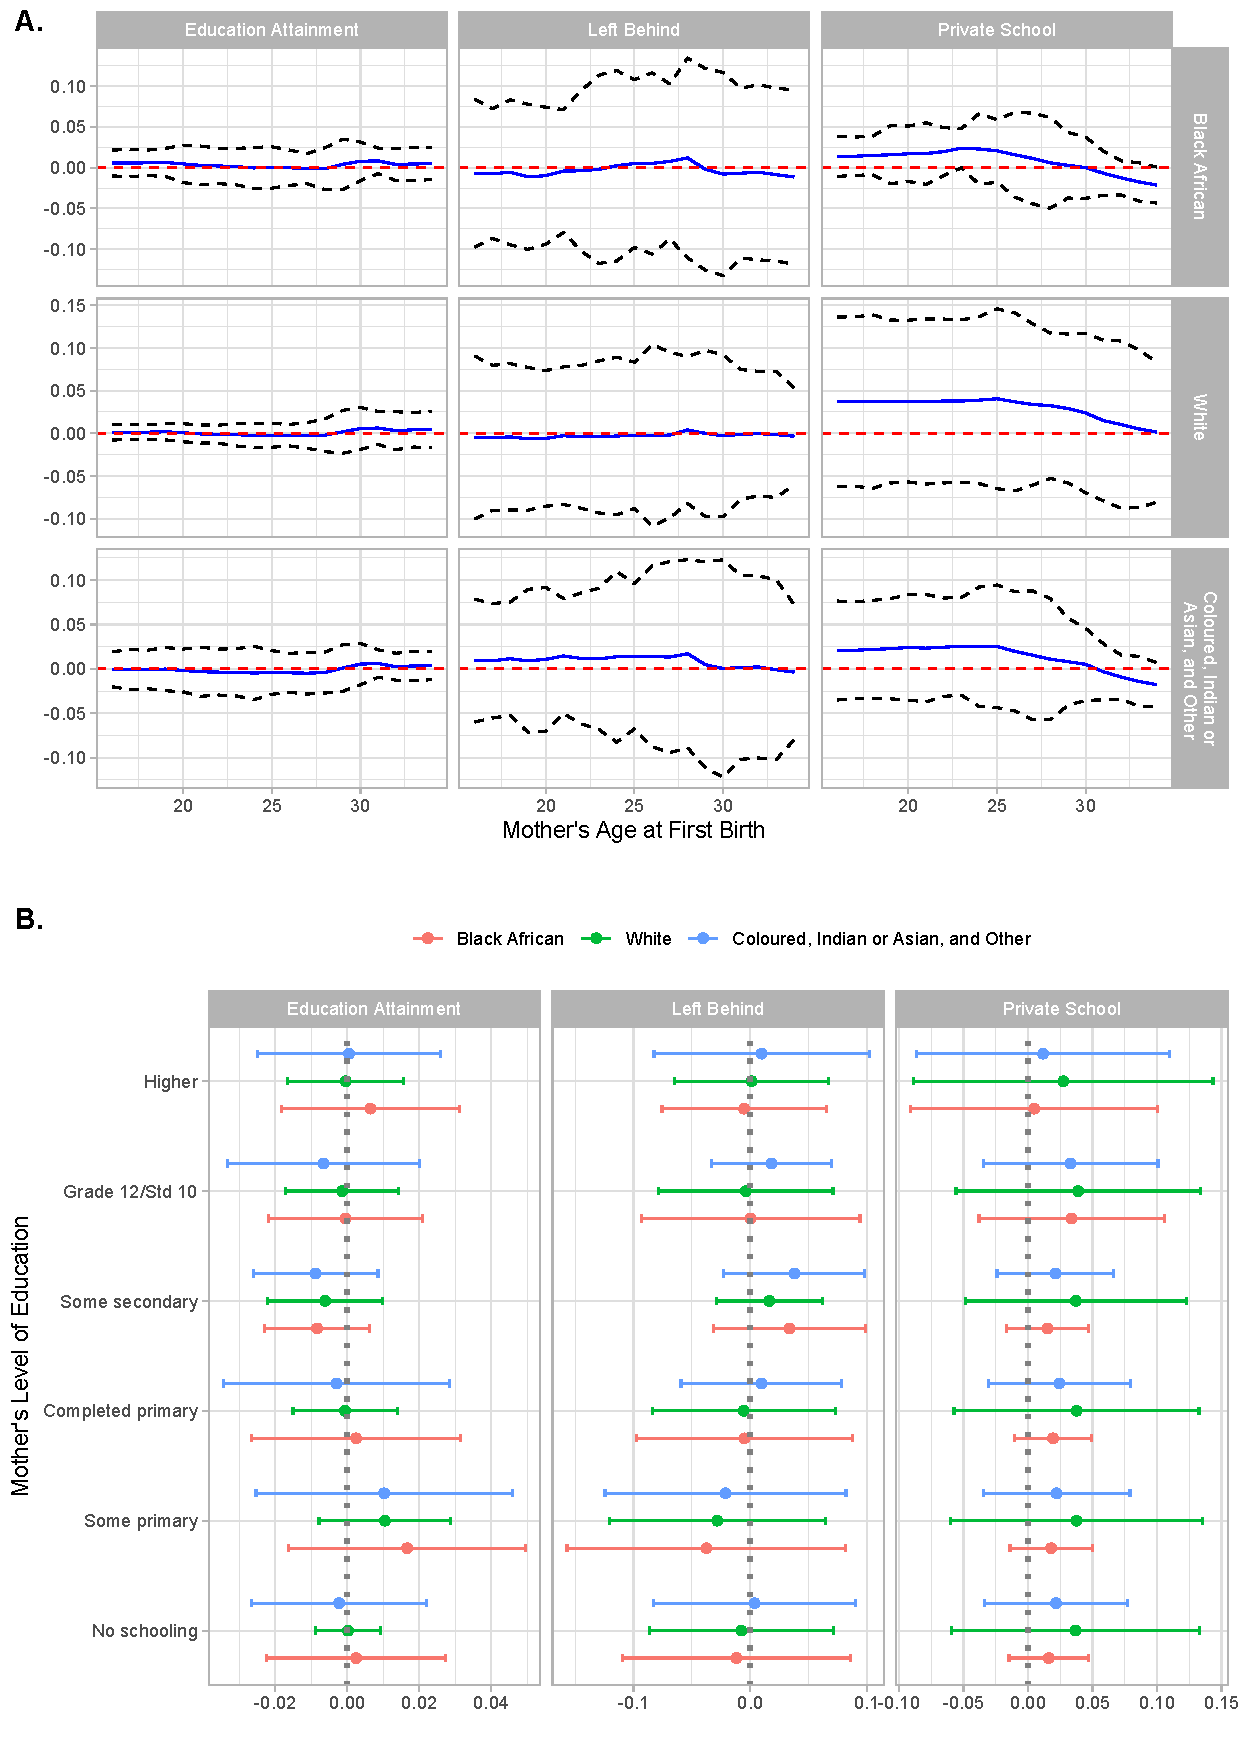
\includegraphics[width=\textwidth]{figures/heter1.pdf}
%\fnote{\textit{Notes:} The above results are based on three forests, one forest for each outcome. Tuning results suggest the default values of the parameters as optimal for each forest. Each forest is based on 5000 trees. }
%\end{figure}
%
%\begin{figure}[p!]
%\centering
%\caption{\label{fig:heter2}Results of Generalized Random Forest Using Same-Sex IV}
%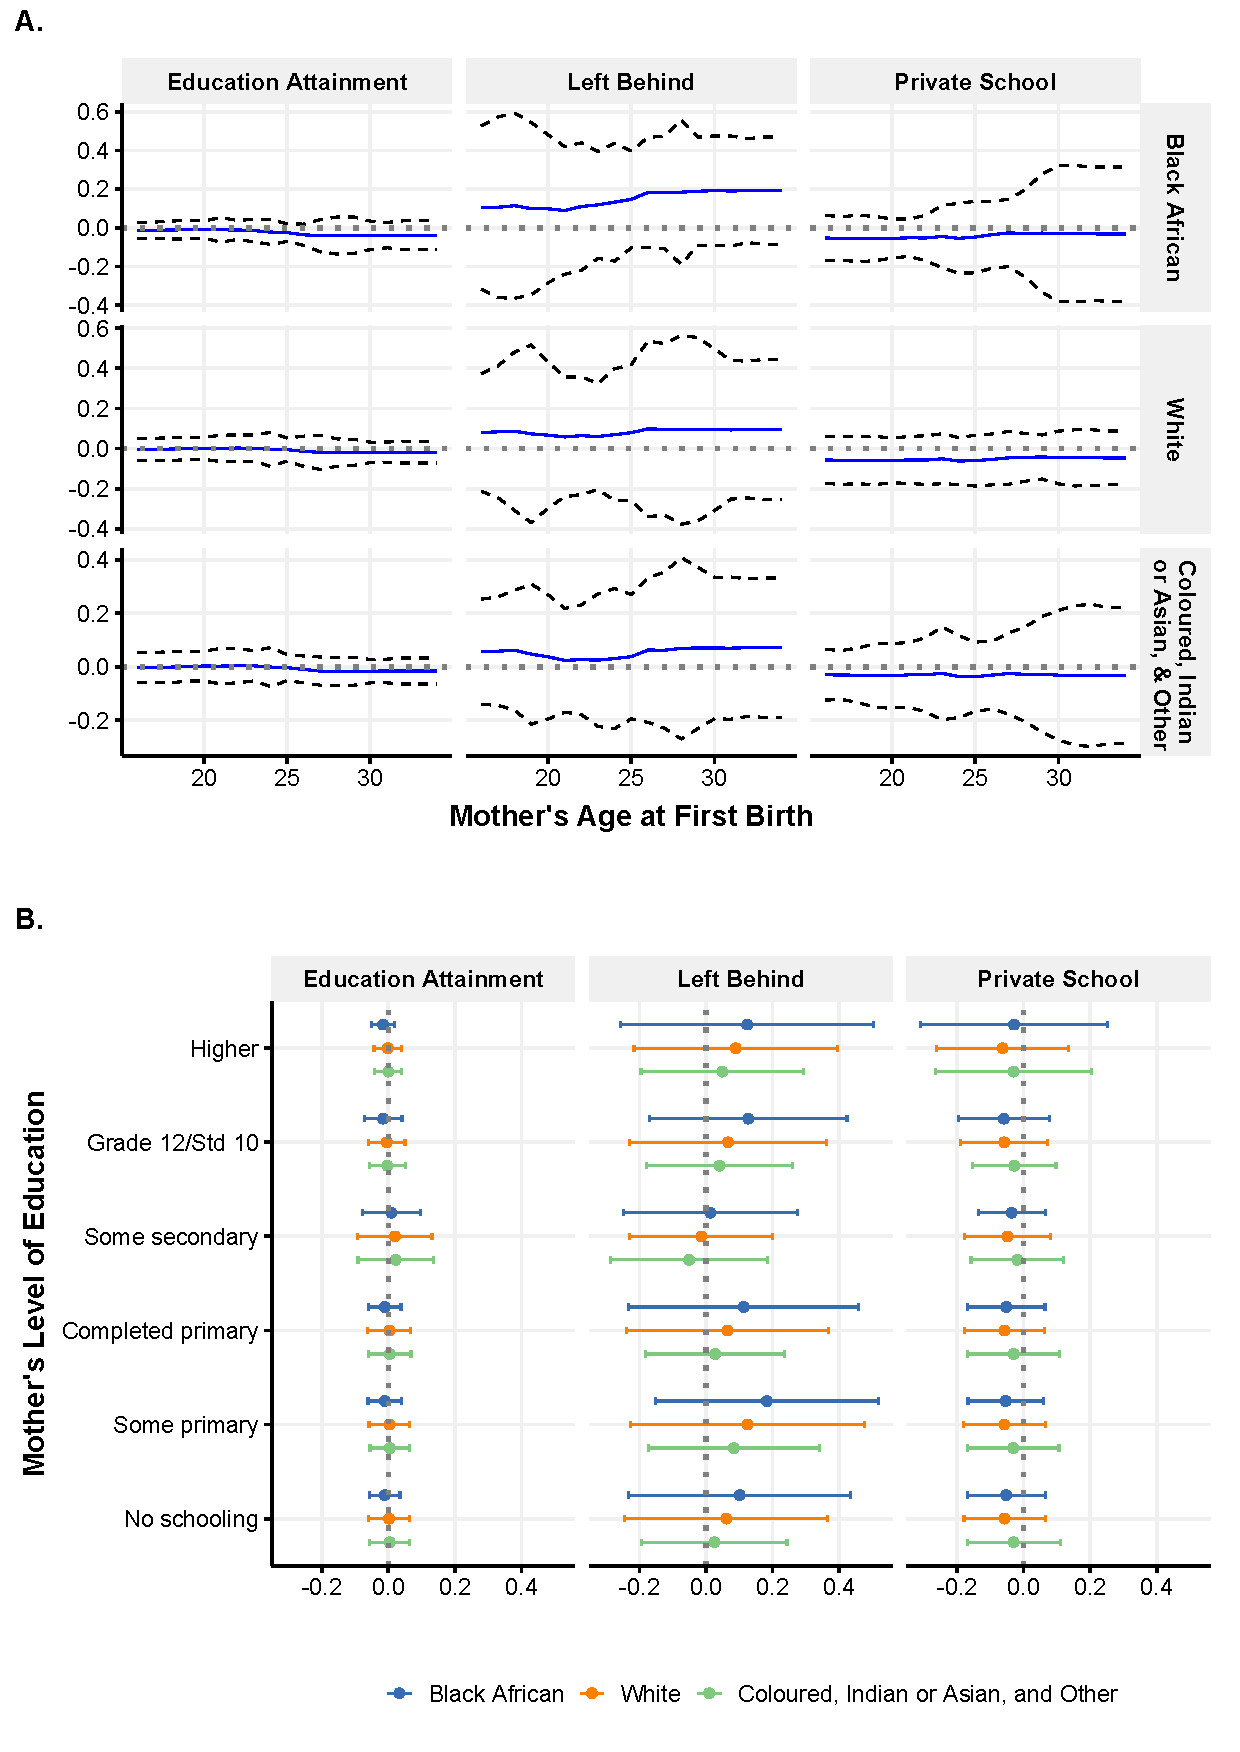
\includegraphics[width=\textwidth]{figures/heter2.pdf}
%\fnote{\textit{Notes:} The above results are based on three forests, one forest for each outcome. The parameters supplied in training each forest were chosen by tuning based on cross-validation. Each forest is based on 5000 trees. }
%\end{figure}

\autoref{fig:heter2} presents the corresponding results obtained using the same-sex instrument (SameSex12). The general pattern of the results is very similar to those presented in \autoref{fig:heter1}. \autoref{fig:heter2}A shows that the effects on educational attainment are almost null for every combination of the mother's age at first birth and her population group, though the confidence intervals are a bit wider than those shown in \autoref{fig:heter1}A. \autoref{fig:heter2}B presents results that parallel those in \autoref{fig:heter1}B. Except for minor distinctions, the results in the two plots are qualitatively identical. Again, the estimates for educational attainment are very precise and seem to indicate an exact null effect. 

In general, the results from a heterogeneity analysis presented above are remarkably consistent in showing no effect of sibling size on any of the outcomes in all the subgroups considered. The estimated effects obtained using two very different instruments (twins birth and sibling sex composition) surprisingly coincide well and in both cases not a single subgroup with a significant effect is identified. This observation bolsters the external validity of these findings; they give us more confidence that the results can be extrapolated to a different population with different characteristics. 

\section{Conclusion}
\label{section:conclude}

This study investigated whether there is a causal relationship between sibship size and the educational attainment of children using census data from South Africa. It employed an IV strategy that relied on a plausible exogenous variation in the number of children due to the birth of twins and preferences for a mixed-sibling sex composition. While both instruments exhibit a strong first-stage and OLS estimates are negative and significant, results from 2SLS regressions provide no evidence of a negative consequences of increased sibship size on educational attainment and other intermediate outcomes. Analysis of effect heterogeneity along multiple dimensions fails to find a significant impact in any of the subsamples and shows that the results do not vary with observable characteristics of the mother. These results are in line with previous research which find no or little effect of family size on child outcomes using similar approaches \parencite[e.g.,][]{Black2005,Black2010,caceres-delpiano_impacts_2006,angrist_multiple_2010,bhalotra_twin_2020}. Hence, this study is the latest in a growing body of empirical literature that challenge the existence of a quantity-quality trade-off in the family.

It is best to exercise considerable modesty in interpreting these results, however. First, the study only focuses on educational attainment of children as measured by enrolment. But enrolment may not translate to learning. Unfortunately, due to data limitations, the study does not consider learning outcomes, as measured by, for example, test scores. It is possible for sibling size not to affect grade attainment, but to adversely affect learning outcomes of children or cognitive development \parencite{Black2010}. Moreover, the study only considers immediate short run outcomes. Though useful, a more important question is the effect on long run outcomes, such as work, earnings, marriage and fertility (particularly, for girls), etc. And finally, the study ignores the effect on the marginal child. That is, the study only focuses on older children and does not consider the effect on a younger child of being born into a larger family. It turns out that identifying effect on the latter is more challenging because of many confounding factors, such as birth order \parencite{Black2005}. The study leaves these issues to future research.  

%\vskip1cm
%
%\subsubsection*{Credit}
%Statistics were done using R 4.1.2 \parencite{RCT2021}, the \texttt{tidyverse} \parencite{Wickham2019}, the \texttt{lubridate} \parencite{Grolemund2011} the \texttt{lfe} \parencite{Gaure2013,Gaure2021} and the \texttt{grf} \parencite{Tibshirani2022} packages. \texttt{statgazer} \parencite{Hlavac2022} and \texttt{xtable} \parencite{Dahl2019} were used to generate \LaTeX~tables. All other packages and the full reproducible code is available online at [].












